\documentclass[twocolumn,a4paper,dvipdfmx]{ieicejsp}
\usepackage[T1]{fontenc}
\usepackage{lmodern}
\usepackage{textcomp}
\usepackage{latexsym}
\usepackage{float}
\usepackage{graphicx}
\usepackage{amsmath, amssymb}
\usepackage{bm}
\usepackage{upgreek}
\usepackage{caption}
\usepackage{booktabs}
\usepackage{multirow}
\usepackage{array}

\captionsetup{font=small}
\setlength{\floatsep}{12pt plus 2pt minus 2pt}
\setlength{\textfloatsep}{14pt plus 2pt minus 2pt}
\setlength{\dblfloatsep}{12pt plus 2pt minus 2pt}
\setlength{\dbltextfloatsep}{14pt plus 2pt minus 2pt}
\setlength{\intextsep}{12pt plus 2pt minus 2pt}

\title{
    {\bf 大喜利のお題画像における文字の扱いとその影響：投稿者の意図による定義から見て決められる文の属性へ}
    {\normalsize \\ Handling Text in Ogiri Prompt Images and Its Effects: From Poster-Intent Definitions to Observable Text Attributes}
}
\author{
    山富 龍 \\ Ryo Yamatomi
}
\affliate{%
    湘南工科大学 大学院 \\
    Graduate University of Shonan Institute of Technology\\
}

\begin{document}
\maketitle
\thispagestyle{plain}
\pagestyle{plain}

\begin{abstract}
大喜利投稿サイト「ボケて」のお題画像の約6割には読める文字があり，その文字が回答者への題であるか，画像の素材の一部であるかによって，ボケの生成に必要な処理が変わる．
本稿では，約682万件のお題画像へのラベルの付与において，画像中の文字をどのように定義し，その定義がラベルの再現性，教師となる視覚言語モデル (Vision-Language Model，VLM) と生徒となる分類器の精度，全データのラベルの分布にどのような影響を与えたかを報告する．
従来の定義では，お題文を「投稿者が回答者に向けて書き加えた文」とし，元の素材の字幕や看板を除いていた．
この定義の下では，誤りの多くがテロップや帯の文字の出所の判断に集中し，VLM は投稿者が加えた文と元の字幕を区別できなかった．
そこで，文字を写っている場所による4つの層と，文の形による5つの形に分け，お題文の有無を属性から規則で導く定義を提案した．
1,620枚の目視ラベルで評価した結果，提案の属性は付け直しで記号の94\%が完全に一致し，選んだ規則で導いたお題文の有無は従来の定義と全データの推定で98.5\%（Cohen の $ \kappa $ 0.90）一致した．
また，規則を変えるだけで，お題文と判定される画像の割合が7.4\%から16.7\%まで変わることを示した．
一方，Qwen3-VL-32B は層を区別できず，教師としての F1 は0.43にとどまり，1,620枚で学習した生徒も既存のパッケージの F1 0.83 に届かなかった．
\par
\noindent
{\bf キーワード} 大喜利，データアノテーション，ラベル設計，視覚言語モデル，画像中の文字
\end{abstract}

\section*{Abstract}
About 60\% of the prompt images on the Japanese Ogiri site Bokete contain readable text, and whether the text is a prompt addressed to the answerers or part of the source material changes the processing needed to generate a witty response.
This paper reports how we defined text in prompt images when annotating about 6.82 million images, and how the definition affected label reproducibility, the accuracy of a vision-language model (VLM) teacher and a student classifier, and the label distribution of the whole dataset.
The previous definition treated a prompt sentence as text added by the poster for the answerers and excluded captions and signs in the source material.
Under this definition, most errors concentrated on judging the origin of captions and bands, and the VLM could not distinguish text added by the poster from original subtitles.
We therefore propose to split text into four layers by where it is placed and five forms by its sentence form, and to derive the presence of a prompt sentence from these attributes by a rule.
On 1,620 manually labeled images, 94\% of the attribute codes were reproduced exactly on relabeling, and the presence of a prompt sentence derived by the selected rule agreed with the previous definition on 98.5\% of the population (Cohen's $ \kappa $ 0.90).
We also show that changing the rule alone moves the share of images with a prompt sentence from 7.4\% to 16.7\%.
However, Qwen3-VL-32B could not distinguish the layers and reached an F1 of only 0.43 as a teacher, and students trained on the 1,620 images did not reach the F1 of 0.83 of the existing package.
\par
\noindent
{\bf Key words} Ogiri, Data Annotation, Label Design, Vision-Language Model, Text in Images

\section{はじめに}
\label{sec_intro}
大喜利は，出題された題目に対して機知に富んだ回答を返す言葉遊びである．
大喜利投稿サイト「ボケて」\cite{ref_bokete}では，投稿者がお題となる画像を掲示し，他の利用者がその画像に対する面白い一言を投稿する．
以下では，お題となる画像をお題画像，利用者が投稿する一言をボケと呼ぶ．
ボケてに蓄積されたお題画像とボケの組は，画像を入力として面白い文を生成するモデルの学習や，ユーモアの分析に利用できる大規模な資源である．
これらの用途では，各お題画像がどの種類に属するかを示すラベルが必要になる．
本研究では，約682万件のお題画像にラベルを付与する方法を構築してきた．

お題画像の扱いを最も難しくしている要素は，画像中の文字である．
お題画像の約6割には読める文字がある．
その文字には，投稿者が回答者に向けて書いた問いや指示もあれば，写真に写った看板，テレビの字幕，漫画の台詞のように，素材に元からある文字もある．
回答者にとって前者は答えるべき題であり，後者は一言を付ける対象の一部である．
したがって，ボケの生成では，文字を読み取るかだけでなく，読み取った文字を題として扱うかを決める必要がある．

従来のラベルでは，題として扱う文字を「お題文」と呼び，投稿者が回答者に向けて書き加えた文と定義していた．
しかし，この定義は投稿者の意図に依存する．
例えば，アニメの画像に重ねた問いの字幕は，元の放送の字幕である場合も，投稿者がテロップ風に書き加えた場合もあり，両者は見た目では区別できない．
このような判断の揺れは，正解のラベルの再現性を下げるだけでなく，教師となる視覚言語モデル (Vision-Language Model，VLM) の判定や，その判定を学習する生徒の分類器の精度も下げる．

本稿では，お題画像の文字の扱いについて，定義の変遷と，各段階の定義がラベルの付与に与えた影響をまとめる．
本稿の貢献は次のとおりである．
\begin{itemize}
    \item ラベルの定義の改訂の過程で，文字の扱いをどのように変えたかを整理し，投稿者の意図に基づく定義の下で生じた誤りの傾向を示す．
    \item 文字を，写っている場所による層と，文の形による形の2軸の属性に分け，お題文の有無を属性から規則で導く定義を提案する．
    \item 提案の属性の再現性，従来の定義との差，規則の選択による全データのラベルの分布の変化を定量的に示す．
    \item 提案の属性を VLM の教師と画像の埋め込みや書き起こしに基づく生徒で学べるかを調べ，移行の障害を明らかにする．
\end{itemize}

本稿の構成は次のとおりである．
\ref{sec_data}章で対象のデータと用語を定義し，\ref{sec_related}章で関連研究を整理する．
\ref{sec_history}章で文字の扱いの変遷を述べ，\ref{sec_intent}章で投稿者の意図に基づく定義の影響を分析する．
\ref{sec_attr}章で文の属性による定義を提案し，\ref{sec_exp}章と\ref{sec_results}章でその評価の方法と結果を示す．
\ref{sec_discussion}章で考察し，\ref{sec_conclusion}章でまとめる．

\section{データと用語}
\label{sec_data}
対象は，ボケてから収集した6,823,270件のお題である．
各お題には1枚の画像があり，ハッシュ値が同じ画像をまとめると6,609,511枚になる．
以下では，ハッシュ値が同じ画像の1枚を代表の画像と呼び，ラベルの評価と全データの推定は代表の画像を単位として行う．

各お題画像には，形式，属性，媒体の3軸のラベルを付与する．
形式は，回答の作り方を表す1つの値であり，カルタ，穴埋め，お題文，通常の4つがある．
カルタは，ひらがな1文字が入った独立した記号があり，そのひらがなから始まる文を投稿する画像である．
穴埋めは，語の代わりに置かれた空欄があり，空欄に入る語を投稿する画像である．
お題文は，画像中の題に答える画像であり，通常はそれ以外の画像である．
属性は，カルタ記号あり，空欄あり，お題文あり，文字ありの複数選択であり，形式はこの順の優先順位で属性から導く．
媒体は，写真，アニメ，ゲーム，マンガ，テキストグラフィック，絵画，イラストの複数選択である．
本稿で扱うのは，属性のうち文字ありとお題文ありの2項目と，お題文ありから導かれる形式のお題文である．

ラベルの付与は，VLM を教師とし，画像の埋め込みに基づく分類器を生徒とする知識蒸留\cite{ref_kd}で行う．
教師は Qwen3-VL\cite{ref_qwen3vl}であり，vLLM\cite{ref_vllm}で推論する．
生徒は，SigLIP 2\cite{ref_siglip2}の画像埋め込みを入力とする多層パーセプトロン (Multi-Layer Perceptron，MLP) である．
生徒は，教師が約4.5万枚に付けたラベルで学習し，全データに適用する．
以下では，この処理をまとめたプログラムをパッケージと呼び，その版を v5.3.0 のように表す．
また，ラベルの定義を記した文書を定義書と呼び，その版を第1版から第6版のように表す．

正解のラベルは，画像を表示して内容を確認できる AI エージェントである Claude Code が，その時点の定義書に従って目視で付与した．
以下では，このラベルを目視ラベルと呼ぶ．
目視ラベルは全て1名の判断者によるものであり，判断者間の一致度は測っていない．

\section{関連研究}
\label{sec_related}
画像とユーモアを扱う研究では，画像に付けた一言の面白さを理解する課題\cite{ref_newyorker}や，ボケてを含む大喜利のデータから回答を生成する課題\cite{ref_oogirigo}が提案されている．
これらの研究は，画像と回答の組を一様に扱うことが多い．
しかし，お題画像には画像中の題に答えるものと画像そのものに一言を付けるものが混在しており，両者を区別しなければ，モデルが画像中の文字を読む必要があるかを評価できない．

画像中の文字を読む課題としては，情景の中の文字を手がかりに質問に答える Visual Question Answering の課題\cite{ref_textvqa,ref_stvqa}が知られている．
これらの課題では，看板や商品の表示のように，写っている世界の中の文字を読むことが主な対象である．
一方，お題画像には，写真の上に重ねた字幕や，画像の外の帯に書いた文が多く含まれ，文字がどこに書かれているかが，その文字の役割を推し量る手がかりになる．
本稿の層の属性は，この違いを明示的に記録するものである．

ラベルの付与では，判断者の間で正解が揺れることが知られており，揺れを誤りとして除くのではなく，データの性質として扱うべきとする議論がある\cite{ref_hlv}．
本稿で扱うお題文の判断の揺れは，判断者の解釈の違いではなく，画像から観測できない投稿者の意図を定義が要求することに由来する．
本稿では，観測できる属性だけでラベルを定義し，解釈に依存する判断を属性からの規則に移すことで，この揺れを扱う．

VLM の判定を高速な分類器に移す方法は，知識蒸留\cite{ref_kd}として知られる．
本研究のパッケージも，Qwen3-VL\cite{ref_qwen3vl}を教師とし，SigLIP 2\cite{ref_siglip2}の埋め込みに基づく生徒を用いる．
本稿では，生徒の入力に日本語の文字認識 (Optical Character Recognition，OCR) の YomiToku\cite{ref_yomitoku}による書き起こしを加えた場合も比べる．

\section{文字の扱いの変遷}
\label{sec_history}
表\ref{tab_history}に，定義書の各版における文字の扱いをまとめる．
文字の扱いは，読める文字の有無を表す文字ありと，題として扱う文字を表すお題文の2つの項目に分かれて改訂されてきた．

\begin{table*}[t]
    \centering
    \caption{定義書の各版における文字の扱い}
    \label{tab_history}
    \small
    \begin{tabular}{>{\centering\arraybackslash}p{0.07\textwidth}>{\raggedright\arraybackslash}p{0.36\textwidth}>{\raggedright\arraybackslash}p{0.25\textwidth}>{\raggedright\arraybackslash}p{0.23\textwidth}}
        \toprule
        版 & お題文の扱い & 文字ありの扱い & 改訂の根拠 \\
        \midrule
        第1版 & 問い，指示，題目の句，状況の設定，名前の列挙．字幕や看板など元からある文字は除く & お題文ありと，その他の文字ありを別の属性とする & -- \\
        第2版 & テロップ，字幕，看板など投稿者が重ねたのではない文は，問いの形でもお題文としない & 同上 & 教師のお題文ありの F1 が約0.63 \\
        第3版 & 形式のお題文のみで表す & お題文ありとその他の文字ありを文字ありに統合．ロゴや透かしは除く & 2項目の境界の誤りが多く，下流の処理は文字を読むかのみを要する \\
        第4版 & テンプレートや無地の背景に書いた主題の文を含めると明記 & ロゴ，透かし，衣服の文字など，読める文字全般とする & 誤りの多くがロゴや小さな文字の扱い \\
        第5版 & お題文ありを空欄やカルタ記号と独立の属性とする．空欄を含む文そのもの，元の素材の文字，吹き出しの台詞を除く & 第4版と同じ & 穴埋めやカルタの画像にも問いの文がある \\
        第6版（提案） & 文字の層と文の形の属性から規則で導く．誰が書いたかを判定に用いない & 層のどれかがあれば文字ありとする & 意図に基づく判断の揺れ \\
        \bottomrule
    \end{tabular}
\end{table*}

文字ありは，改訂のたびに観測できる基準へ近づいた．
第1版と第2版では，お題文ありとその他の文字ありを別の属性としていたが，2つの項目の誤りの多くは，テロップを投稿者が重ねた文とみなすかの判断にあった．
下流の処理で必要なのは文字を読み取るかの判断であり，題であるかは形式のお題文で表せるため，第3版で2つの項目を文字ありに統合した．
第3版の文字ありはロゴや透かしを除いていたが，教師はこれらを含めて回答し，定義と教師の判定がずれていた．
そこで第4版では，読める文字があれば文字ありとした．
この改訂では，ロゴや衣服の文字を問う別の短い質問を教師に加え，カルタ記号のない画像に限ってその回答を文字ありに加えた．
その結果，実データの目視ラベルに対する教師の文字ありの F1 は0.954から0.971に上がった．
第4版の目視ラベルに対して，パッケージの文字ありは実データで適合率0.94，再現率0.99であり，文字ありの判定に大きな課題は残っていない．

一方，お題文は，投稿者が回答者に向けて書いた文という意図に基づく定義を第1版から保ち，境界の規則を版ごとに書き足してきた．
第2版では，元からある文字の範囲をテロップや字幕にまで広げた．
この改訂により，教師のお題文ありの F1 は約0.63から0.79に上がった．
第5版では，空欄やカルタ記号のある画像にも投稿者が書いた問いがあることから，お題文ありを形式から独立した属性とした．
このとき，話者を付けた台本，分類の名札だけの見出し，書き写した既存の歌詞，テンプレートの定型の見出しをお題文から除く規則を加えた．
これらの規則は，いずれも文字の出所や書き手の意図を判断の根拠としている．

\section{投稿者の意図に基づく定義の影響}
\label{sec_intent}
本章では，第4版と第5版のお題文の定義の下で行った評価から，意図に基づく定義が教師，生徒，全データのラベルに与えた影響を示す．

\subsection{評価の方法}
お題文ありの画像は全データの約8\%と少ないため，無作為に抽出した目視ラベルだけでは正例が不足する．
そこで，パッケージの予測で代表の画像を層に分け，層ごとに無作為に抽出して目視ラベルを付け，層の重みで全データの値を推定した．
層 $ h $ に属する代表の画像の数を $ N_h $，そのうち目視ラベルを付けた画像の数を $ n_h $ とすると，層 $ h $ の画像 $ i $ の重みは $ w_i = N_h / n_h $ である．
目視ラベルを $ y_i \in \{0, 1\} $，予測を $ \hat{y}_i \in \{0, 1\} $ とすると，全データの適合率 $ P $ と再現率 $ R $ の推定値は(\ref{eq_weighted_pr})で表される．

\begin{equation}
    P = \frac{\sum_{i} w_i y_i \hat{y}_i}{\sum_{i} w_i \hat{y}_i}, \quad
    R = \frac{\sum_{i} w_i y_i \hat{y}_i}{\sum_{i} w_i y_i}
    \label{eq_weighted_pr}
\end{equation}

\noindent
F1 は $ P $ と $ R $ の調和平均であり，95\%区間は層ごとの復元抽出によるブートストラップで求めた．
評価には，第4版の目視ラベルを付けた1,020枚と，第5版のお題文ありの評価のために新たに抽出した600枚を用いた．
1,020枚は，評価用データの640枚と，実データの無作為抽出160枚および層別抽出220枚からなる．
600枚は，パッケージの形式の予測とお題文ありの生徒の確率で分けた9層からの抽出であり，お題文ありの正例を多く含む．

\subsection{教師への確認の質問}
第4版の段階で，教師は元の素材の文字をお題文とする誤りが多かった．
定義の説明に「元からある文字は大きくてもお題文ではない」と書き足すと，実データでお題文と誤る画像はかえって13枚から18枚に増えた．
一方，教師がお題文とした画像に限って「投稿者が回答者に向けて書いた問い，指示，題目の句があるか」を別の質問で確かめると，実データでの誤りは13枚から4枚に減り，実データでの教師のお題文の F1 は0.769から0.873に上がった．

しかし，この確認の質問は，お題文と通常の区別には働いていなかった．
確認の質問を目視ラベルのある1,020枚の全てに問うと，お題文の適合率は0.20，再現率は1.00であった．
「はい」と答えた割合は，目視でお題文の画像で96/96，穴埋めで192/259，カルタで50/69，通常で141/596であった．
確認の質問は，題であるかよりも，投稿者が書き加えたらしい文の有無に反応していた．
また，生徒がお題文とした画像に限ると，確認の質問は目視ラベルのある画像で一度も「いいえ」と答えず，全データでも対象の567,345枚のうち0.7\%の判定しか変えなかった．

\subsection{第5版のお題文ありと VLM}
第5版でお題文ありを独立の属性としたため，穴埋めとカルタの画像328枚にお題文ありの目視ラベルを付け直したところ，30枚がお題文ありであった．
表\ref{tab_qwen_v5}に，この正解に対する教師の F1 を示す．
評価用は1,020枚のうちの最終評価用の320枚，実データは無作為抽出と層別抽出の380枚の重み付きの値である．

\begin{table}[t]
    \centering
    \caption{第5版のお題文ありに対する教師の F1 と推論の速さ}
    \label{tab_qwen_v5}
    \small
    \begin{tabular}{lccc}
        \toprule
        モデルと指示 & 枚/秒 & 評価用 & 実データ \\
        \midrule
        8B，確認の質問 & 18.9 & 0.43 & 0.39 \\
        8B，定義と手順 & 12.7 & 0.57 & 0.56 \\
        32B，確認の質問 & 9.7 & 0.52 & 0.53 \\
        32B，定義と手順 & 6.0 & 0.76 & 0.75 \\
        \bottomrule
    \end{tabular}
\end{table}

8B のモデルは，定義と判断の手順を詳しく与えてもお題文ありと答えすぎた．
誤りの多くは，空欄を含む文そのもの，テレビの字幕，漫画の台詞をお題文とするものであった．
32B のモデルに定義と手順を与えると，除外の条件をおおむね守れたが，F1 は0.75前後にとどまった．
32B のモデルを全データに適用すると約12.8日を要するため，その判定を4.5万枚の教師ラベルとして生徒に学習させ，パッケージ v5.3.0 に組み込んだ．

\subsection{第5版の評価と残った誤り}
600枚のうち層別抽出の420枚で，パッケージ v5.3.0 のお題文ありの F1 は0.831であり，お題文ありの全データの割合は7.9\%と推定された．
同じ判断者による90枚の付け直しの一致は，一致率0.978，Cohen の $ \kappa $\cite{ref_kappa} 0.95 であった．
不一致の2枚は，話者を付けた台本と書き写した歌詞であり，いずれも付け直しの時点で境界の規則を定めたことによる差であった．

残った誤りは，文字の出所の判断に集中した．
穴埋めやカルタと予測され，お題文ありの生徒の確率が0.3以上の層では，目視でお題文ありの画像は35\%にとどまった．
この層のお題文なしの画像の多くは，空欄を含む1文だけの画像や，空欄を含む歌詞，記事，名札の見出し付きの問題文であった．
また，形式が通常と予測された画像には，全データで約3.0万枚のお題文ありの見逃しがあると推定された．
生徒の確率が0.7以上の通常の画像でも，お題文ありは56\%であった．
これらの画像の多くは，写真の上下の帯や写真に重ねた文字の画像であり，人物の台詞の字幕と，投稿者が加えた問いや状況の文が同じ見た目になる．
32B のモデルも，この中のお題文なしの74枚のうち33枚をお題文ありと答えた．

以上から，意図に基づく定義の下では，教師と生徒の誤りの多くが，画像から観測できない文字の出所の判断に集中していたといえる．
境界の規則を書き足すことで目視ラベルの再現性は保たれたが，同じ見た目の画像に異なるラベルを求めるため，教師と生徒が学ぶべき区別そのものが画像に現れない．

\section{文の属性による定義}
\label{sec_attr}
本章では，お題文ありを直接付与する代わりに，画像から観測できる文の属性を付与し，お題文ありを属性から規則で導く定義を提案する．
提案の定義では，誰が書いたか，題のつもりで書いたか，既存の歌詞や台詞の引用であるかを記録しない．

\subsection{文字の層}
文字の層は，画像中の読める文字がどこにどう書かれているかを表す複数選択の属性である．
場面の文字は，写っている世界の中にある文字であり，看板，商品の表示，本の表紙，スクリーンショットの画面の中の文字を含む．
透かし，ロゴ，署名，ボケてのテンプレートに印刷された定型の見出しも，位置によらず場面の文字とする．
吹き出しは，漫画やイラストの吹き出しと語りの枠の中の文字であり，吹き出しのない，人物の脇に描き込まれた台詞を含む．
重ねた文字は，写真や絵の上に重ねた文字であり，テレビの字幕やテロップ，写真への書き込みを含む．
元の放送の字幕か投稿者が加えたものかは問わない．
余白の文字は，写真や絵の外にある文字であり，画像の上下左右の帯や枠，無地の背景，テンプレートの文字欄に書いた文字を含む．
写真や絵の領域の上にあれば重ねた文字，外にあれば余白の文字とし，帯の下地が不透明で絵を隠している場合は余白の文字とする．
文字ありは，4つの層のどれかがある場合に真とする．

\subsection{文の形}
文の形は，重ねた文字と余白の文字について，それぞれの層にどの形の文があるかを表す複数選択の属性である．
場面の文字と吹き出しの文の形は記録しない．
空欄を含む文は，空欄を含む文と，空欄を含む文章のまとまりであり，まとまりは空欄のない文を含んでいても全体をこの形とする．
問いは疑問の形の文であり，「もし〜たら」で始まる条件の形の文を含む．
指示は回答者への依頼や命令の形の文である．
題目の句は，「〜あるある」「こんな〜は嫌だ」のように大喜利の題となる名詞句や定型の句である．
その他の文は，上記のどれでもない平叙文，台詞，題名，名前，項目の名札などである．
空欄を含む文の判定を先に行い，空欄を含むまとまりの中の問いや指示は問いや指示としない．

図\ref{fig_examples}に，層と形の例を示す．
図の記号は，層を s（場面の文字），b（吹き出し），o（重ねた文字），m（余白の文字），形を k（空欄を含む文），q（問い），i（指示），t（題目の句），x（その他の文）で表し，コロンの後に層の形を示したものである．
図\ref{fig_examples}(d)の元のアニメの字幕と，図\ref{fig_examples}(e)のテロップ風に書き加えた問いは，いずれも重ねた文字の問いとなる．

\begin{figure}[t]
    \centering
    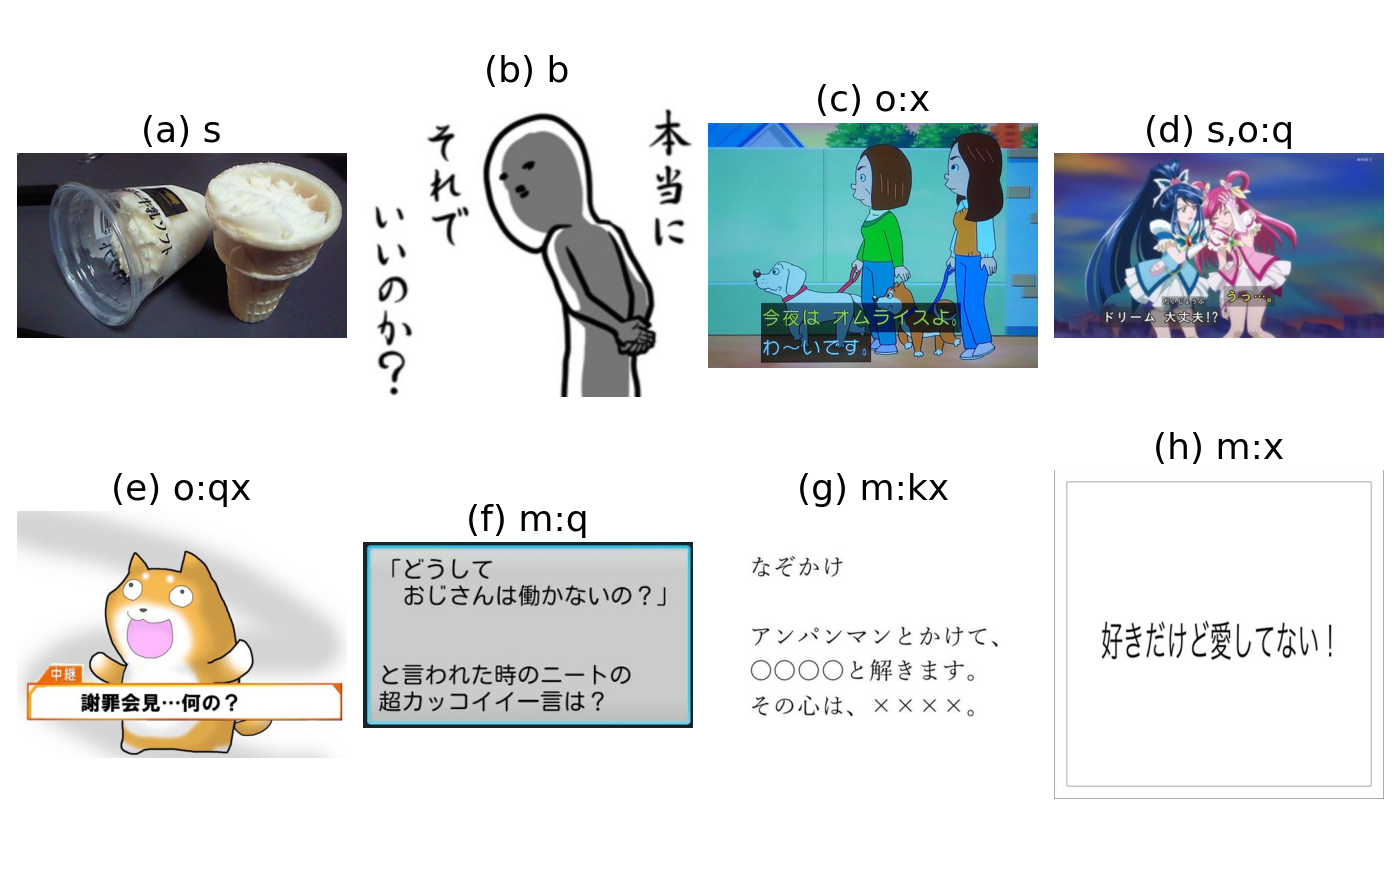
\includegraphics[width=\columnwidth]{figures/fig_examples.png}
    \caption{文の属性の例．(a) 商品の表示，(b) 人物の脇に描かれた台詞，(c) アニメの字幕の台詞，(d) アニメの字幕の問い，(e) テロップ風に書き加えた問い，(f) 枠の中の問い，(g) 名札と空欄を含む文，(h) 無地の背景の平叙文}
    \label{fig_examples}
\end{figure}

\subsection{お題文ありの規則}
重ねた文字に形 $ f $ の文がある場合に1，ない場合に0をとる変数を $ o_f $，余白の文字について同様の変数を $ m_f $ とする．
ここで $ f \in \{k, q, i, t, x\} $ は文の形の記号である．
問い，指示，題目の句のどれかが重ねた文字か余白の文字にあることを表す $ a $ を(\ref{eq_task})で定義する．

\begin{equation}
    a = \bigvee_{f \in \{q, i, t\}} \left( o_f \lor m_f \right)
    \label{eq_task}
\end{equation}

\noindent
お題文ありを導く規則として，(\ref{eq_rules})の4つを考える．

\begin{align}
    r_0 &= a, \nonumber \\
    r_1 &= a \lor m_x, \nonumber \\
    r_{1b} &= a \lor \left( m_x \land \lnot m_k \right), \nonumber \\
    r_2 &= r_1 \lor o_x
    \label{eq_rules}
\end{align}

\noindent
規則 $ r_0 $ は，問い，指示，題目の句だけを題とみなす．
規則 $ r_1 $ は，余白に書かれたその他の文も題とみなす．
余白のその他の文は，無地の背景に書いた台詞の書き出しや状況の文であることが多く，回答者はその文を読んで回答を作るためである．
規則 $ r_{1b} $ は，余白に空欄を含む文がある場合に，余白のその他の文を根拠としない．
この場合のその他の文は，名前，分類の名札，題名のように，空欄を埋めるための見出しであることが多いためである．
規則 $ r_2 $ は，重ねた文字の台詞や字幕もお題文とみなす．
本稿では $ r_{1b} $ を既定の規則とする．
規則は属性から計算するため，属性を付け直さずに規則を変更でき，規則ごとの違いを同じ目視ラベルで比べられる．

重ねた文字の問い，指示，題目の句は，$ a $ を通じて，元の字幕であるかによらずお題文ありとなる．
投稿者が写真に重ねた問いと元の字幕の問いは見た目で区別できず，どちらを除いても一方を誤るためである．
比較のため，$ a $ から重ねた文字の形を除いた規則 $ r_{1b}' = \bigvee_{f \in \{q, i, t\}} m_f \lor ( m_x \land \lnot m_k ) $ も評価する．

\section{評価の方法}
\label{sec_exp}
\begin{figure*}[t]
    \centering
    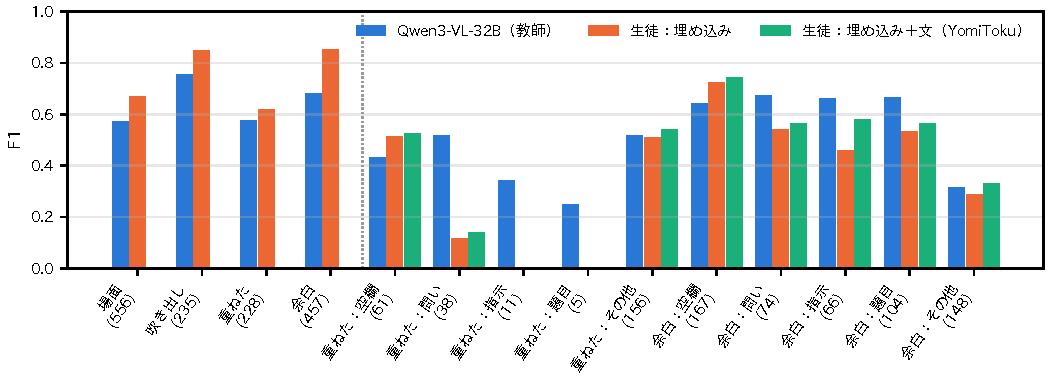
\includegraphics[width=\textwidth]{figures/fig_attrs.pdf}
    \caption{属性ごとの F1（1,620枚）．生徒は5分割の交差検証の分割外の予測であり，層の属性は埋め込みのみで学習した}
    \label{fig_attrs}
\end{figure*}

\subsection{目視ラベル}
\ref{sec_intent}章の1,020枚と600枚を合わせた1,620枚に，提案の属性の目視ラベルを付けた．
画像は並べ替えて番号だけを付けた一覧の画像にし，パッケージの予測と第5版の目視ラベルを伏せて付与した．
再現性を確かめるため，1,620枚から無作為に選んだ90枚を番号を付け直して別の一覧にし，同じ判断者が付け直した．
全データの推定値は，600枚に(\ref{eq_weighted_pr})の重みを用いて求め，1,020枚は学習と重みなしの値にのみ用いた．
2つのラベルの一致は，重み付きの一致率と Cohen の $ \kappa $ で評価した．

\subsection{教師}
教師は Qwen3-VL-32B-Instruct の FP8 量子化版であり，入力の画素数の上限は802,816画素である．
4つの層の有無，重ねた文字と余白の文字の文の形，両層の書き起こしを JSON の形式で答えさせた．
また，書き起こしだけを答えさせる指示を，同じモデルと Qwen3-VL-2B-Instruct に問うた．
YomiToku でも全ての文字を書き起こしたが，YomiToku は層を区別しない．

\subsection{生徒}
生徒は，属性ごとのロジスティック回帰であり，1,620枚の5分割の交差検証で分割外の予測を求めた．
入力は，パッケージが保存した SigLIP 2 の1,152次元の画像埋め込みと，書き起こした文の文字の1〜3-gram の Term Frequency-Inverse Document Frequency (TF-IDF) の特徴である．
文の特徴は，教師の書き起こしでは重ねた文字と余白の文字を別の語彙とし，YomiToku の書き起こしでは全ての文字を1つの語彙とした．
層の属性は埋め込みだけで学習し，文の形の属性は埋め込み，文，両方の3通りで学習した．
正則化の係数は，埋め込みで $ C = 0.05 $，文で $ C = 4 $，両方で $ C = 1 $ とし，正例と負例の重みを釣り合わせた．
確率が0.5以上の場合に真とした．

お題文ありの予測は2通りで求めた．
1つ目は，生徒の層と形の予測を(\ref{eq_rules})に代入して導く方法である．
2つ目は，規則で導いた目視のお題文ありを，属性を経ずに直接学習する方法である．
比較の基準は，第5版の定義で学習したパッケージ v5.3.0 のお題文ありである．
パッケージの生徒は約4.5万枚の教師ラベルで学習しており，1,620枚で学習した生徒とは学習の量が異なる．

\section{結果}
\label{sec_results}
\subsection{属性の頻度と再現性}
全データの推定では，場面の文字は35.0\%，吹き出しは14.3\%，重ねた文字は8.3\%，余白の文字は12.1\%の画像にあり，いずれかの層がある画像は58.7\%であった．
この割合は，パッケージが文字ありとした代表の画像の割合と一致する．
付け直した90枚では，層と形の記号の完全一致は94.4\%であった．
層ごとの $ \kappa $ は0.95〜1.00であり，規則で導いたお題文ありの $ \kappa $ は $ r_{1b} $ で1.00，$ r_1 $ で0.97，$ r_2 $ で0.92であった．
不一致は，小さな場面の文字の見落とし，テレビの字幕の層の判断，名札や曲名をその他の文として記録するかの判断にあった．

\subsection{規則とお題文ありの割合}
表\ref{tab_shift}に，規則ごとに導いたお題文ありと，第5版の目視のお題文ありとの一致を示す．
v5 のみと v6 のみは，それぞれ一方の定義でのみお題文ありとなる画像の割合である．

\begin{table}[t]
    \centering
    \caption{規則で導いたお題文ありと第5版の目視ラベルとの一致（全データの推定）．第5版のお題文ありの割合は7.93\%である}
    \label{tab_shift}
    \small
    \begin{tabular}{cccccc}
        \toprule
        規則 & 一致率 & $ \kappa $ & 割合 & v5 のみ & v6 のみ \\
        \midrule
        $ r_0 $ & 98.1\% & 0.864 & 7.40\% & 1.23\% & 0.70\% \\
        $ r_1 $ & 97.3\% & 0.839 & 10.31\% & 0.15\% & 2.52\% \\
        $ r_{1b} $ & 98.5\% & 0.904 & 8.95\% & 0.23\% & 1.26\% \\
        $ r_{1b}' $ & 98.6\% & 0.906 & 8.31\% & 0.52\% & 0.89\% \\
        $ r_2 $ & 91.1\% & 0.592 & 16.67\% & 0.10\% & 8.84\% \\
        \bottomrule
    \end{tabular}
\end{table}

規則を変えるだけで，お題文ありの割合は7.40\%から16.67\%まで変わった．
$ r_{1b} $ は第5版と最もよく一致し，$ \kappa $ は0.904であった．
$ r_2 $ は第5版から大きく離れ，お題文ありの割合が約2倍になった．
重ねた文字の台詞や字幕は，第5版では多くがお題文なしであったためである．

1,620枚で $ r_1 $ と $ r_{1b} $ の判定が分かれた画像は34枚であり，いずれも余白に空欄を含む文とその他の文がある画像であった．
そのうち24枚は第5版でお題文なしであり，キャラクターの紹介の画面の名前，「なぞかけ」の名札，映画の題名などであった．
残りの10枚は第5版でお題文ありであり，空欄の文とは別に置いた状況の文や見出しの画像であった．

重ねた文字に問い，指示，題目の句がある画像は，1,620枚で53枚であった．
そのうち第5版でお題文ありは18枚，お題文なしは35枚であり，お題文なしの35枚の多くは，アニメや映画の台詞の字幕が問いの形になったものであった．
全データの推定では，これらの画像は全体の0.65\%であり，第5版でお題文ありが0.28\%，お題文なしが0.37\%であった．
$ r_{1b} $ と $ r_{1b}' $ の第5版との $ \kappa $ は0.904と0.906であり，重ねた文字の問いを含めるかは，第5版との一致ではほぼ決まらない．

\subsection{教師と生徒の属性の精度}
図\ref{fig_attrs}に，1,620枚での属性ごとの F1 を示す．
横軸は属性であり，左の4項目が層，右の10項目が層ごとの文の形である．
括弧内は正例の数である．
縦軸は目視ラベルに対する F1 である．

教師の層の F1 は0.57〜0.76であり，いずれの層でも再現率が0.87以上，適合率が0.64以下であった．
教師は層を広く真と答え，場面の文字を真とした誤り651枚のうち370枚は文字の層がない画像，余白の文字の誤り355枚のうち235枚はスクリーンショットや看板などの場面の文字の画像であった．
層をまとめた文の形の F1 は，問い0.78，空欄を含む文0.77，指示0.73，題目の句0.71，その他の文0.55であり，教師は文字がどこにあるかよりも，どの形の文があるかを答える方が得意であった．

生徒は，余白の文字と吹き出しを埋め込みだけでいずれも F1 0.85 で学べ，教師を上回った．
一方，場面の文字は0.67，重ねた文字は0.62にとどまった．
文の形は，余白の空欄を含む文が0.72であったほかは，埋め込みだけでは0.0〜0.54であった．
文の特徴を加えると多くの形で F1 が上がったが，重ねた文字の問い，指示，題目の句は正例が5〜38枚と少なく，ほとんど学べなかった．
教師の書き起こしを YomiToku の書き起こしに替えても，形の F1 の差は小さかった．

\subsection{導いたお題文ありの精度}
表\ref{tab_odai}に，$ r_{1b} $ で導いた目視のお題文ありを正解としたときの，各方法のお題文ありの F1 を示す．
参考として，第5版の目視のお題文ありを正解とした値を併記する．

\begin{table}[t]
    \centering
    \caption{お題文ありの F1（全データの推定）．括弧は95\%区間}
    \label{tab_odai}
    \footnotesize
    \setlength{\tabcolsep}{2pt}
    \begin{tabular}{lcc}
        \toprule
        方法 & 正解 $ r_{1b} $ & 正解 第5版 \\
        \midrule
        パッケージ v5.3.0 & 0.828 [0.79, 0.86] & 0.829 \\
        教師の属性から導く & 0.434 [0.36, 0.53] & 0.398 \\
        生徒の属性：埋め込み & 0.650 [0.55, 0.76] & 0.653 \\
        生徒の属性：＋文（32B） & 0.730 [0.64, 0.83] & 0.732 \\
        生徒の属性：＋文（YomiToku） & 0.773 [0.70, 0.84] & 0.783 \\
        直接学習：埋め込み & 0.751 [0.63, 0.86] & 0.733 \\
        直接学習：＋文（32B） & 0.785 [0.67, 0.89] & 0.755 \\
        \bottomrule
    \end{tabular}
\end{table}

教師の属性から導いたお題文ありは，F1 が0.434にとどまった．
層の誤りが規則に伝わり，お題文ありを広く真としたためである．
1,620枚で学習した生徒は，いずれもパッケージ v5.3.0 に届かなかった．
属性を経る生徒では，埋め込みに YomiToku の書き起こしを加えた場合が最も高く，F1 は0.773であった．
パッケージ v5.3.0 は，正解を $ r_{1b} $ としても第5版としても F1 が約0.83 であり，$ r_{1b} $ の定義が第5版に近いことを示している．

図\ref{fig_curve}に，学習に用いた画像の数と分割外の F1 の関係を示す．
横軸は5分割のうち学習に用いた画像の数であり，縦軸は1,620枚の重みなしの F1 である．
余白の文字は約300枚で F1 0.8 に達した．
一方，直接学習したお題文ありは約650枚以降で伸びが小さく，問いとその他の文は1,296枚でも0.5前後であった．

\begin{figure}[t]
    \centering
    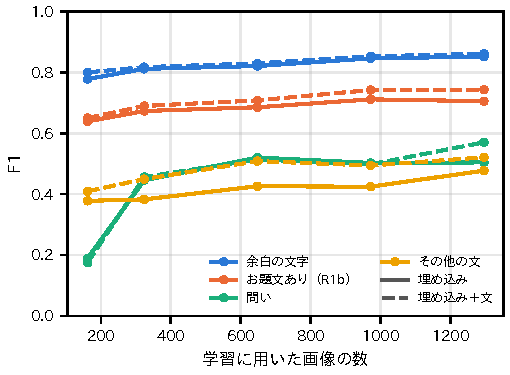
\includegraphics[width=\columnwidth]{figures/fig_curve.pdf}
    \caption{学習に用いた画像の数と分割外の F1．実線は埋め込みのみ，破線は埋め込みと教師の書き起こしの文を入力とした生徒である}
    \label{fig_curve}
\end{figure}

\subsection{書き起こしの費用}
表\ref{tab_speed}に，1,620枚での書き起こしと属性の問い合わせの速さと，パッケージが文字ありとした代表の画像の全てに適用した場合の見積もりを示す．
いずれも単一の GPU での値である．

\begin{table}[t]
    \centering
    \caption{書き起こしの速さと，文字ありの代表の画像約388万枚への適用の見積もり}
    \label{tab_speed}
    \small
    \begin{tabular}{lcc}
        \toprule
        方法 & 枚/秒 & 見積もり \\
        \midrule
        32B，属性と書き起こし & 2.7 & 約16.8日 \\
        32B，書き起こしのみ & 7.5 & 約6.0日 \\
        2B，書き起こしのみ & 21.2 & 約2.1日 \\
        YomiToku & 6.2 & 約7.2日 \\
        \bottomrule
    \end{tabular}
\end{table}

\section{考察}
\label{sec_discussion}
\subsection{定義の観測可能性とラベルの再現性}
第5版のお題文ありは，境界の規則を書き足すことで，同じ判断者の付け直しで $ \kappa $ 0.95 を得ていた．
提案の属性も付け直しで層の $ \kappa $ が0.95以上，規則で導いたお題文ありの $ \kappa $ が0.92〜1.00であり，意図を記録しなくても再現性は下がらなかった．
両者の違いは，再現性そのものではなく，ラベルの根拠が画像に現れるかにある．
第5版では，同じ見た目の字幕の問いに，元の字幕であればお題文なし，投稿者が加えた文であればお題文ありという異なるラベルを求めていた．
提案の属性では，見た目が同じ画像には同じ属性が付くため，判断の揺れは属性ではなく規則の選択として明示される．
実際に，テロップを含めるかという判断は，$ r_1 $ と $ r_2 $ の比較として，ラベルを付け直さずに評価できた．

\subsection{規則の選択がデータに与える影響}
規則の選択によって，お題文ありの割合は7.40\%から16.67\%まで変わった．
お題文ありは，ボケの生成で画像中の文を題として読む処理を適用する対象を決めるため，この差は下流の処理の対象の数に直接影響する．
$ r_{1b} $ は第5版との差が最も小さく，第5版のお題文ありを用いた既存の分析との互換性を保てる．
一方，$ r_{1b} $ では，余白に空欄を含む文と並ぶ状況の文が，問い，指示，題目の句の形でない限りお題文の根拠にならない．
また，重ねた文字の問いを含めるかは，第5版との一致ではほぼ決まらず，台詞の字幕が問いの形のものを題とみなしてよいかという判断に帰着する．
この判断は，画像だけでなく，その画像に付いたボケが問いに答えているかによって確かめられる可能性がある．

\subsection{教師と生徒への影響}
提案の属性への移行の主な障害は，教師の精度である．
Qwen3-VL-32B は，文の形はある程度答えられたが，文字がどの層にあるかを区別できず，層の誤りが規則を通じてお題文ありの誤りに伝わった．
一方，生徒は余白の文字と吹き出しを埋め込みだけで学べており，層の判断は画像の見た目に現れている．
このことから，層は少数の目視ラベルで学習した生徒に任せ，教師には層をまとめた文の形だけを問う構成が考えられる．
文の形は，1,620枚の目視ラベルでは学習が不足し，学習曲線も頭打ちに近かったため，数万枚規模の教師ラベルが必要と考えられる．
書き起こしの文を生徒に加えると精度は上がったが，文字ありの画像の全てに適用するには，最も速い方法でも約2.1日を要する．

\subsection{限界}
本研究には次の限界がある．
第1に，目視ラベルは全て同じ判断者によるものであり，再現性は同じ判断者の付け直しの一致である．
人どうしの一致は測っていない．
第2に，提案の属性の評価に用いた1,620枚は，第5版の評価のために誤りの疑われる画像を多く選んだ集合を含み，重みなしの値は全データより食い違いが多く出る．
第3に，比較の基準のパッケージは約4.5万枚の教師ラベルで学習しており，1,620枚で学習した生徒との比較は学習の量の差を含む．

\section{おわりに}
\label{sec_conclusion}
本稿では，大喜利のお題画像における文字の扱いの変遷と，その影響をまとめた．
読める文字の有無を表す文字ありは，改訂のたびに観測できる基準に近づき，適合率0.94，再現率0.99で判定できるようになった．
一方，題として扱う文字を表すお題文は，投稿者の意図に基づく定義を保ったため，教師と生徒の誤りが文字の出所の判断に集中した．
そこで，文字を写っている場所による4つの層と，文の形による5つの形に分け，お題文ありを属性から規則で導く定義を提案した．
提案の属性は同じ判断者の付け直しで記号の94\%が一致し，既定の規則 $ r_{1b} $ で導いたお題文ありは第5版と全データの推定で98.5\%一致した．
また，規則の選択だけでお題文ありの割合が7.40\%から16.67\%まで変わることを示した．
一方，Qwen3-VL-32B は層を区別できず，1,620枚で学習した生徒も既存のパッケージに届かなかった．
今後は，層を生徒に任せて教師には文の形だけを問う構成で教師ラベルを増やすこと，人どうしの一致を測ること，ボケの内容から規則の妥当性を確かめることが課題である．


\vspace{-1mm}
\begin{thebibliography}{99}

    \bibitem{ref_bokete}
    ボケて (bokete), https://bokete.jp/, (2026年11月閲覧).

    \bibitem{ref_newyorker}
    J. Hessel, et al., ``Do Androids Laugh at Electric Sheep? Humor ``Understanding'' Benchmarks from The New Yorker Caption Contest,'' Proc. ACL, 2023.

    \bibitem{ref_oogirigo}
    S. Zhong, et al., ``Let's Think Outside the Box: Exploring Leap-of-Thought in Large Language Models with Creative Humor Generation,'' Proc. CVPR, 2024.

    \bibitem{ref_textvqa}
    A. Singh, et al., ``Towards VQA Models That Can Read,'' Proc. CVPR, 2019.

    \bibitem{ref_stvqa}
    A. F. Biten, et al., ``Scene Text Visual Question Answering,'' Proc. ICCV, 2019.

    \bibitem{ref_hlv}
    B. Plank, ``The ``Problem'' of Human Label Variation: On Ground Truth in Data, Modeling and Evaluation,'' Proc. EMNLP, 2022.

    \bibitem{ref_kd}
    G. Hinton, O. Vinyals, and J. Dean, ``Distilling the Knowledge in a Neural Network,'' arXiv:1503.02531, 2015.

    \bibitem{ref_qwen3vl}
    Qwen Team, ``Qwen3-VL Technical Report,'' arXiv:2511.21631, 2025.

    \bibitem{ref_vllm}
    W. Kwon, et al., ``Efficient Memory Management for Large Language Model Serving with PagedAttention,'' Proc. SOSP, 2023.

    \bibitem{ref_siglip2}
    M. Tschannen, et al., ``SigLIP 2: Multilingual Vision-Language Encoders with Improved Semantic Understanding, Localization, and Dense Features,'' arXiv:2502.14786, 2025.

    \bibitem{ref_yomitoku}
    K. Kinoshita, ``YomiToku: AI-OCR for Japanese documents,'' https://github.com/kotaro-kinoshita/yomitoku, 2024.

    \bibitem{ref_kappa}
    J. Cohen, ``A Coefficient of Agreement for Nominal Scales,'' Educational and Psychological Measurement, vol. 20, no. 1, pp. 37--46, 1960.

\end{thebibliography}


\end{document}
